% Autor: Kryštof Glos

\chapter*{Úvod}
Procedurálně vytvářený obsah v herním průmyslu je velmi důležitou součástí her už po několik let. Mnoho her postavených na této vlastnosti už se prosadilo na trhu a stále více se uplatňuje. Náhodné vytváření obsahu se používá například na tvoření herních map, věcí v místnosti, skládání různých dopředu vytvořených místností tak aby vznikla jedinečná mapa, zkrátka skoro všude. 

Hlavním důvodem používání náhodně vytvořeného obsahu je možnost opakovaného hraní stejné hry, bez toho aby se hra stala nezáživnou. V budoucnu se procedurální generování rozhodně neztratí a naopak se bude ještě více využívat v různých odvětvích. Cíl této práce je vytvořit jedinečnou 2D hru z pohledu z hora, která právě takové náhodné vytváření bude používat. Hra je o přežití a ovládání skupiny domorodců a nastolení míru na ostrově. V kapitole \ref{Teorie} je detailně popsáno náhodné generování a různé metody,v kapitole \ref{solution} je vysvětleno jaké způsoby budou nejlepší k řešení, jak byla práce naplánována a proč. V kapitole \ref{realization} je popsaný způsob jakým byla hra řešena, použité metody a jejich význam.

\chapter{Vytváření obsahu v herním světě} 
\label{Teorie}
Ve světě her jsou dvě možnosti jak přistupovat ke tvoření obsahu, jedním z těchto způsobů je tradiční nebo také mechanické. \hyperref[traditional]{Mechanické generování} je nejjednodušší, ale také nejpracnější. Další možností vytváření obsahu je pomocí metod implementující náhodné, nebo také \hyperref[procedural]{procedurální generování obsahu}. (anglicky Procedural Generation dále jen PG) je složitější na implementaci, avšak jakmile je implementované tak už žádné navrhování úrovní není třeba, takové úrovně však mohou mít chyby pokud nejsou správně ošetřeny. (například nedostupné místnosti, rostlina na vodě, atd.)

Hry které mají pouze dvě dimenze se nazývají 2D. (z anglického two dimensions) Je mnoho žánrů 2D her, RPG (role playing game) hry na hrdiny s příběhem, strategií, Co-op (kooperační) které jsou postavené na spolupráci více hráčů, survival (hry o přežití), colony-sim (z anglického colonization simulation) které mají simulovat kolonizaci ovládanou hráčem a tak dále. Tato bakalářská práce se zabývá hrou žánru colony-sim. Je mnoho způsobů jak vyvíjet takovou hru, nejčastěji se používají takzvané \hyperref[enginy]{herní enginy}, které takové vyvíjení hry ulehčují a jsou na to stavěné.


\section{Způsoby generování obsahu}
V této části porovnáme mechanické generování obsahu s procedurálním, vysvětlíme co je lepší kdy použít a jaké známe metody pro procedurální generování. Následující tři body popisují faktory, které je třeba zvážit při rozhodování, zda bude využita nějaká procedurální metoda na generování, nebo bude lepší použít manuální design úrovní a obsahu:
\begin{description}
	\item[Žánr tvořené hry] Při vytváření například takové FPS hry, u které záleží hlavně na ovládání a souboji hráče proti hráči, není třeba vytvářet mapy a další obsah procedurálně. Většinou stačí vytvořit například pouze jednu úroveň a na to není potřeba požívat procedurální generování. Při hrách které závisí na okolí, surovinách a přežití kde každá okolnost nějak ovlivňuje hráče, už procedurální generování hraje větší roli. Zároveň pro vytváření obsahu jako je text, může být PG velmi obtížnou volbou, neboť v RPG hrách bývá textová část velmi důležitá a generování textu je stále dost obtížné
	\item[Opakovaná hratelnost] Některé hry jsou dělané tak že čím déle hráč hraje stejnou úroveň(anglicky level) tím více se zlepšuje a je za to například odměňován je právě manuální tvoření úrovní lepší než procedurální. Naopak u jiných her, které mají úrovně procedurálně generované, většinou hráč danou úroveň zvládne, pokračuje na další a nepředpokládá se že se k ní bude ještě vracet.
	\item[Aspekt designu hry] Jestliže hra závisí z velké části na jedné úrovni s jejími mechanikami, vlastnostmi a obsahem, pak je lepší ji vytvářet mechanicky a doladit všechny vlastnosti a interakce s hráčem.
\end{description}


\subsection{Mechanické generování obsahu}
\label{traditional}
Mechanický typ generování je jedním z nejobvyklejších tvoření obsahu ve hrách. Používá se převážně v žánrech, jako je RPG (Role Play Game), RTS(Real Time Strategy) a další, ve kterých pozice objektů a struktura mapy hraje velkou roli a bez lidské tvorby by nebylo dosaženo potřebných výsledků. Toto tvoření lze interpretovat jako proces u něhož se návrhář za pomoci různých nástrojů, které postupně aplikuje, snaží dosáhnout požadovaného výsledku. Jde tedy o metodu ručního vytváření obsahu kde designér, nebo grafik navrhuje a postupně vytváří úroveň, či jinou část hry tak, aby vyhovovala potřebám, ať už se jedná o pozici stromu, nebo o to co hráči sděluji NPC.
	
Proces takového vytváření obsahu pro hry se dá zjednodušeně představit na příkladu. Uvažujme například truhláře vyrábějícího stůl, který také používá různé nástroje na zhotovení nábytku. Aplikováním těchto nástrojů na materiál postupně vytváří výsledný stůl. Nástroje a suroviny, které si na počátku celého procesu vybral, určí možné výsledky, takže výsledkem jeho práce nemůže být třeba obraz.

Díky tomuto přístupu nehrozí nesrovnalosti ve výsledku, například se nemůže stát že určitá část mapy bude nedostupná, nebo úplně nesmyslná. Další výhodou je, že výsledek bude přesně takový jak byl naplánovaný, avšak takovéto tvoření je u větších her, kde je nutná opětovná hratelnost, velmi časově náročné.

\subsection{Procedurální generování obsahu}
\label{procedural}
Tento typ vytváření obsahu se používá ve více žánrech, ale asi nejznámější z hlediska generování map je Roguelike, kde každá nová hra má unikátní náhodnou mapu. PG se ovšem nepoužívá pouze na generování map, ale také na vytváření objektů, jako jsou stromy, textury, animace, text a další. Procedurální generování obsahu není to stejné jako, jak se mnozí domnívají, náhodné generování obsahu.
\begin{figure}[h]
	\centering
	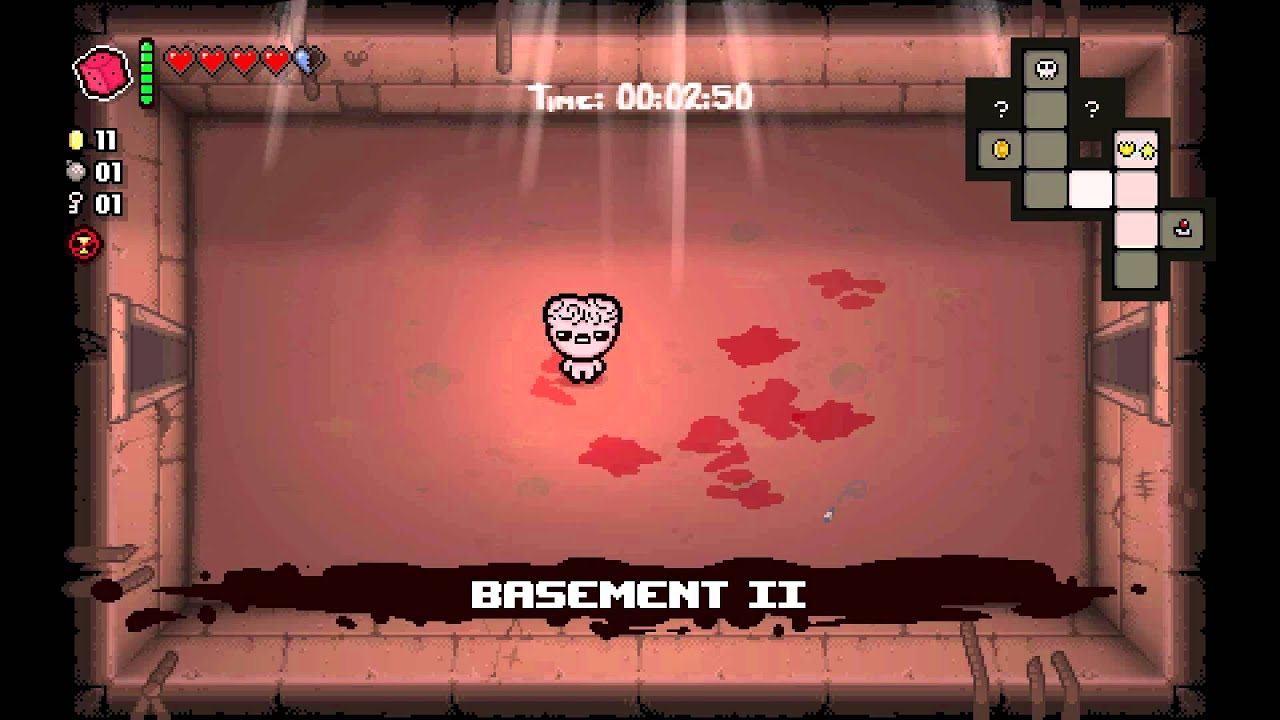
\includegraphics[scale=0.33]{obrazky-figures/BindingOfIsaac.jpg}
	\caption{Příklad hry Roguelike žánru jménem Binding of Isaac, vpravo nahoře je vidět mapa dungeonu, která je procedurálně vygenerovaná, i takto může PG vypadat.}
\end{figure}


V zásadě je to proces obrácený jak u mechanického generování obsahu. Uživatel sice stále definuje různé nástroje, které jsou použity pro vytváření obsahu, ale nikoli pro své vlastní použití, ale naopak je vytváří pro algoritmus. Uživatel dále určuje pravidla podle kterých se generátor musí řídit tak, aby se dobral kýženého výsledku.

\subsubsection{Příklad procedurálního generování lesů}
\label{proceduralExample}
Pro lepší představu uvedu příklad. Program má funkci procedurálního generátoru lesů na mapě, cílem tohoto programu je náhodně naskládat stromy s rozumnými rozestupy od sebe. Pomocí mechanického generování obsahu by designér jednoduše přidával modely stromů do té doby, dokud by mapa neodpovídala představám návrháře a nesplňovala by potřeby herního designu. V případě procedurálního generování, je nutné definovat nástroje, což je v tomto příkladě schopnost přidávat stromy na mapu a pravidla, jako například kolik stromů je potřeba aby algoritmus vysázel, kam program může jednotlivé stromy pokládat a jaké jsou minimální rozestupy mezi nimi. Pravidla a nástroje nám tím pádem jednoznačně definují množinu potenciálních výsledku.

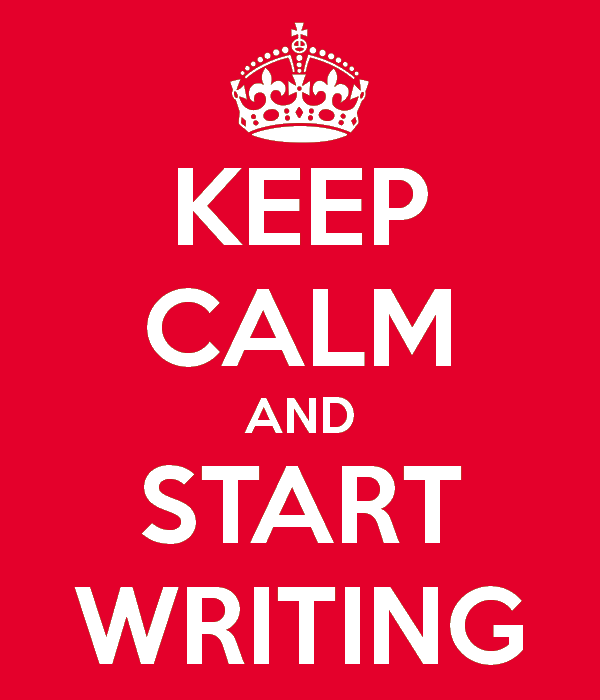
\includegraphics[scale=0.3]{obrazky-figures/keep-calm.png}
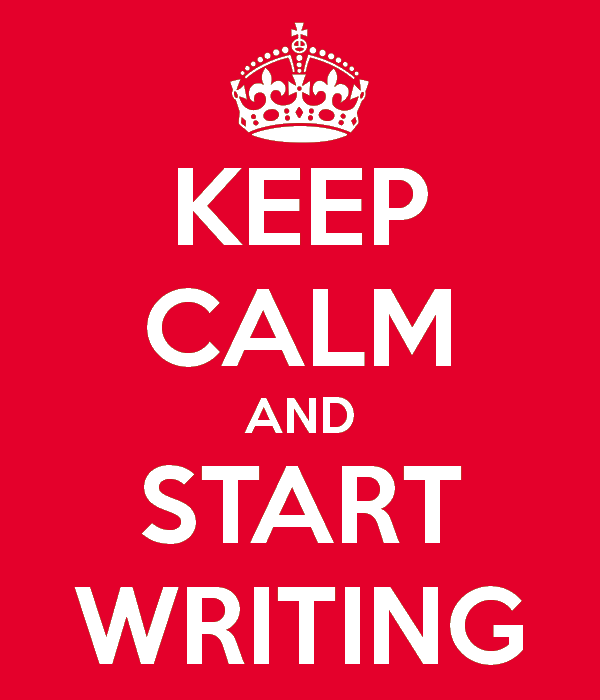
\includegraphics[scale=0.3]{obrazky-figures/keep-calm.png}

\todo{dva obrázky, jeden se stromy moc u sebe a druhý lepší při použití více pravidel}

\section{Procedurální generování v herním průmyslu}
\label{metody}
Algoritmů na generování obsahu existuje mnoho, každý používá jiné nástroje, ale všechny se musí podrobovat pravidlům která stanovuje programátor a podle kterých se řídí. Je více způsobů a míst kde se dá PG uplatnit, různé způsoby a důvody jsou popsány v této kapitole.

\subsection{Text}
Skoro všechny hry používají text. Z důvodu že každá informace v textu musí odpovídat realitě, je nutno velké množství omezení pro generování. Například když je v textu informace že král je mrtvý \cite{liuDeep}, musí být toto tvrzení pravdivé.

Velkým plusem procedurálního generování textu je vyprávění \cite{madoc59000}, takto vytvořené příběhy jsou často kreativnější a zajímavější, než ty co by vytvořil člověk, neboť lidé mají sklony psát příběhy které již slyšeli, nebo ze svých zkušeností, což dost omezuje nápady.

\subsection{Krajina a úrovně}
Nejvíce obvyklý obsah který se ve hrách generuje a který je zároveň hlavním zaměřením této práce, jsou krajiny a úrovně. Generování lokací, úrovní, nebo obsahu mapy lze jak u 2D her, tak u 3D her. Za úroveň nebo oblast lze označovat otevřené, třeba krajina s lesy, i uzavřené prostranství, vnitřek budovy, nebo jeskyně. Tato část PG je rozvedená a podrobněji popsaná v následující kapitole \ref{Krajina}.

\subsection{Textury}
Textury jsou snad skoro ve všech 3D a velké části 2D her. Zároveň se jedná o obsah který má nejméně omezení pro generování. Jednou z nejčastějších metod, která se používá na tvoření textur, je \todo{odkaz na perlinův šum} Perlinův šum, který je detailněji popsán v kapitole \todo{tady a tady}.

\subsection{Zvuky a hudba}
Většina her má soundtrack a zvukové efekty. Soundtrack většinou nemá nijak zvlášť přísná pravidla, ale zvukové efekty musejí být výstižné a odpovídající akci v daný moment. 

Jukebox \cite{Dhariwal2020JukeboxAG} je model který dokáže generovat hudbu se zpěvem v originální nezpracované formě zvukových dat, s délkou v řádu minut, i s určením žánru a vokálního stylu. Modelů jako je tento již existuje více, avšak zatím to nejsou plně hodnotné soundtracky pro hry a ještě chvíli potrvá, než bude možné jednoduše vygenerovat hudbu a efekty pro hru pomocí pouhého nástroje.

\pagebreak

\chapter{Procedurální generování}
Tato kapitola popisuje různé metody a použití procedurálního generování v herním průmyslu, do detailu popisuje PG krajiny, generování fraktálů.

Roden and Parberry \cite{FromArtistry} pojmenovávají tento druh algoritmů \textit{amplifikační algoritmy (amplification algorithms)}, přijímají menší množství vstupních informací, které zpracují a vracejí větší objem dat na výstupu. Hendrikx et al. \cite{Hendrikx} pojímají procedurální generování jako alternativu k mechanickému navrhování obsahu, ale kladou důraz na zdokonalování a přidávání parametrů umožňujících zásah návrháře do takto vygenerovaných objektů.

\section{Celulární automaty pro PG}
\label{celular}
Celulární automaty se ve hrách používají intenzivně zejména pro modelování týkajícího se systémů v prostředí, jako jsou teplo, oheň, déšť, tlak a exploze. Zatím podle průzkumu nejsou známé žádné hry, které by postavili generování celého 2D herního světa, pouze pomocí celulárních automatů. Momentálně existují webové stránky, které možnost generování malých map pomocí mřížek navrhují, ale není jich mnoho a neexistuje žádné spolehlivé ohodnocení těchto algoritmů. \cite{articleCellular}

Původně byly CA vymyšleny Johnem Von Neumannem jako formální model sebereprodukujících se organismů. šlo o dvou-dimenzionální celulární automat, kde každá buňka, tzv. cell, je malý čtverec na velkém čtverečkovaném papíru. Každá buňka má dva možné stavy, černý a červený, které jsou určeny jejich sousedstvím. V John Von Neumannově teorii, je sousedství tvořené čtyřmi přilehlými čtverci a na obrázku níže jsou vyznačeny červenou barvou. \cite{Gong2017}

Nejznámější celulární automat byl vytvořen v roce 1970 britským matematikem Johnem Hortonem Conwayem, který se jmenoval Game Of Life. Stejně jako Von Neumannův byl i tento automat dvou-dimenzionální a mohli nabývat pouze hodnot živá, nebo mrtvá. Využívá Moorovo sousedství, které oproti Von Neumannově považuje za sousední buňky všech osm přilehlých, vyobrazené na obrázku. Fungování automatu je následovné, buňka zůstává naživu, pokud má dvě, nebo tři sousedící buňky živé. Což simuluje, že buňka nepřežije pokud je osamělá, ale zároveň pokud je okolí přeplněné organismy, tak je utlačována. Další pravidlo je, že pokud je libovolná buňka mrtvá, může se "narodit", pokud jsou v sousedství alespoň tři živé buňky. Toto pravidlo má simulovat rození, kde každá buňka musí mít tři rodiče. Automat díky těmto jednoduchým pravidlům dokáže vytvářet až překvapivě hezké výsledky a opravdu vypadá jako živý organismus. \cite{Gong2017}

\begin{figure}[h]
	\centering
	\begin{subfigure}{0.475\textwidth}
		\centering
		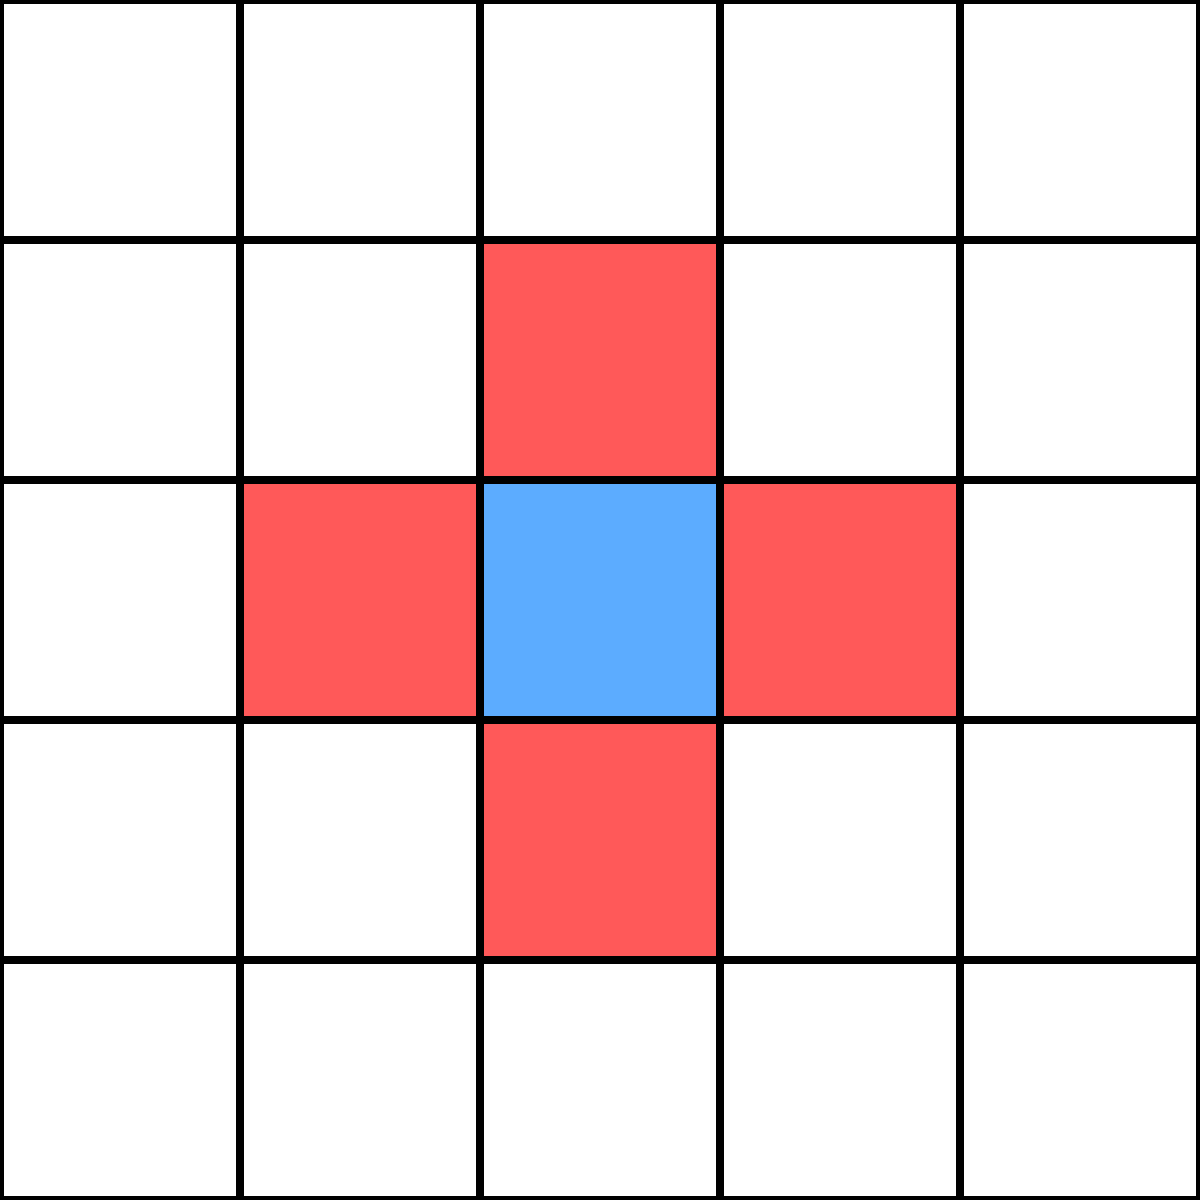
\includegraphics[scale=0.1]{obrazky-figures/Von_neumann_neighborhood.svg}
		\caption{Von Neumannovo sousedství}
	\end{subfigure}
	\begin{subfigure}{0.475\textwidth}
		\centering
		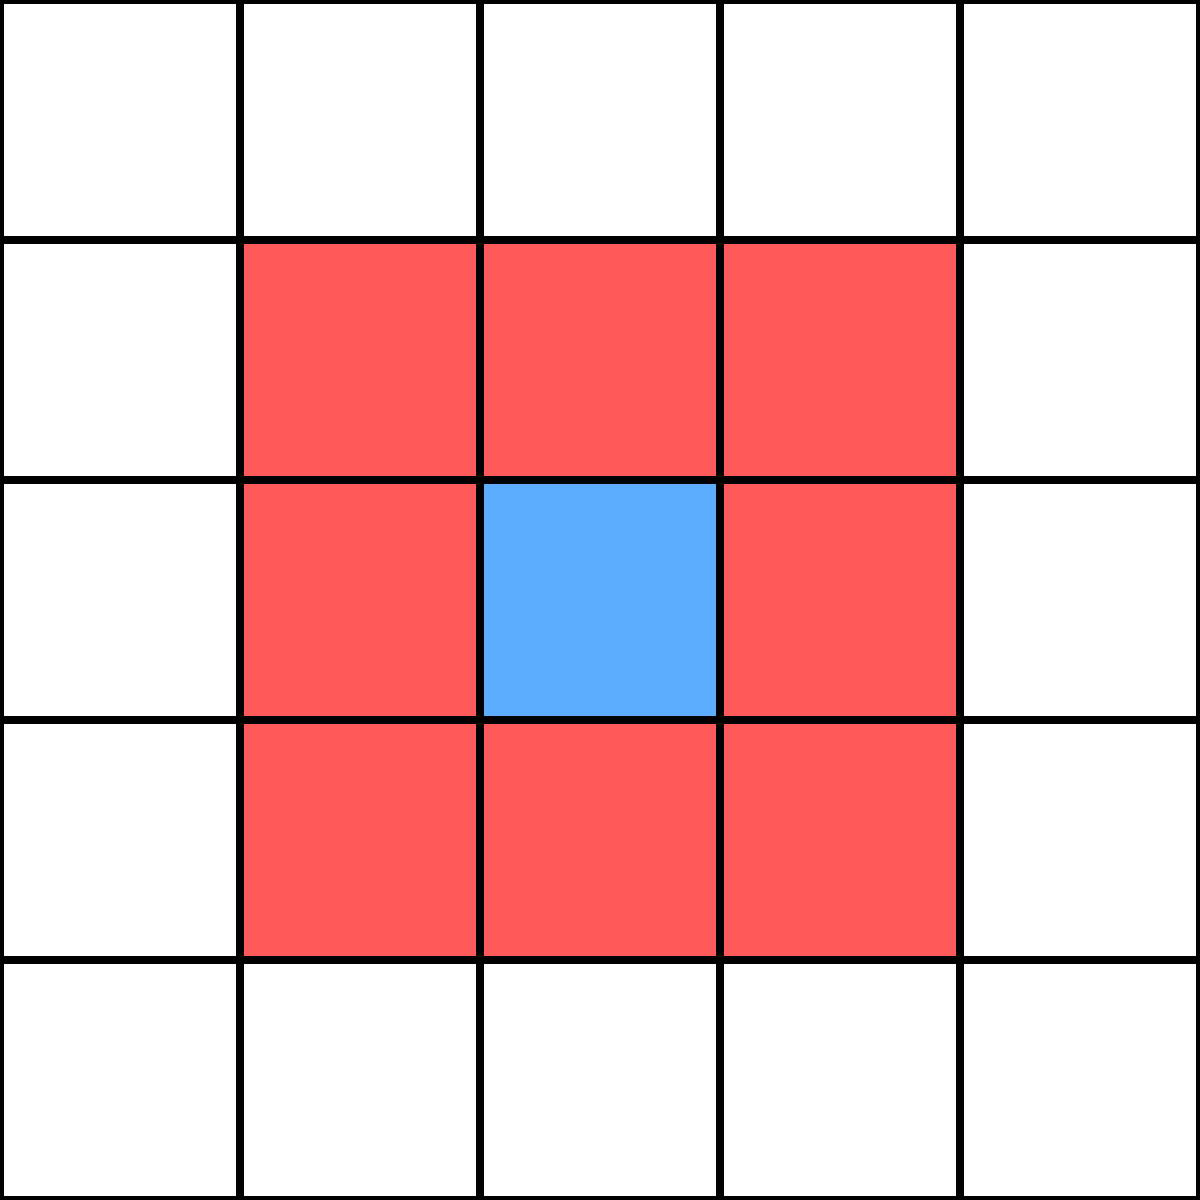
\includegraphics[scale=0.1]{obrazky-figures/Moore_neighborhood.svg}
		\caption{Moorovo sousedství}
	\end{subfigure}
	\caption{Sousedství podle Von Neumanna a dle Moora}
\end{figure}

\section{Procedurální generování krajiny}
\label{Krajina}
Procedurální generování krajiny se řadí ke složitějším tématům PG. Je tomu tak hlavně kvůli tomu, že se k tomuto typu generování většinou používají výškové mapy (height maps) \todo{idealne odkaz na cast kde se popisuji vyskove mapy}, které se skládají z bitových map odstínů šedé, ve kterých se výška udává pomocí právě odstínu šedé barvy daného pixelu. Většinou se používá postup, při kterém platí, že čím světlejší je pixel, tím větší je výška. Jakmile jsou pixely ohodnoceny, jsou tři různé způsoby jak postupovat:
\begin{itemize}
	\item ruční vykreslování textur,
	\item aplikování textur na ručně vytvořené regiony podle výšky,
	\item vygenerování textur po analyzování výšek na vygenerované výškové mapě.
\end{itemize}
Ruční vykreslování textur je jednoduché, ale výsledkem je nedostatečné rozlišení, nebo příliš velká bitmapa. Druhá metoda je podobná, nakreslí se barvy na určitá místa, kam si designer myslí že by se mohly hodit hory, řeky, nebo země. Jedná se o docela obvyklou metodu, která přináší velice kvalitní výsledky, ale stále se jedná o manuální techniku.

Třetí metoda používá data height mapy a vypočítává jakou texturu použít na které místo. Nízké hodnoty (tmavší místa) se používají jako oceány, střední hodnoty se vyhodnocují jako země/tráva a na vysoké hodnoty (světlá místa) se nanášejí textury hor nebo kamení. Při generování ve 3D hrách lze ještě započítávat takzvané sklony (slopes), díky kterým je možné oddělovat vyšší plochy od nižších pomocí dalších textur například kamene.

Vzhledem k tomu že první dva postupy vyžadují mechanické vykreslování buď barvy, nebo textur on designéra, nedá se o nich mluvit jako o čistě procedurálních metodách. Naopak postup třetí tomuto popisu zcela odpovídá, neboť kompletně závisí na height mapě a není nutná žádná akce návrháře \cite{madoc59000}.

\pagebreak
\paragraph*{Generování oblastí lze rozdělit následovně:}
\begin{description}
	\item[Vytváření půdorysu] Tímto pojmem se rozumí vytváření samotné podstaty oblasti. Zahrnuje vytvoření země, moří, řek, hor, atd. Všechny tyto oblasti jsou otevřeného typu. Také můžeme rozumět pod generováním půdorysu i vytváření uzavřeného typu oblastí, například rozložení jednotlivých místností jeskynního komplexu, vytvoření bludiště a jeho cest. 
	
	\item[Přidání vegetace a objektů] Tento bod v podstatě navazuje na předchozí, je potřeba abychom měli vytvořený půdorys, aby bylo kam přidávat a rozmísťovat další objekty. Jedná se o bod do kterého spadá vegetace, budovy, atd. Programu se zadávají různá omezení na množství vegetace, místa kam který objekt lze přidávat a další omezení.
\end{description} 

\begin{figure}[h]
	\centering
	\begin{subfigure}{0.475\textwidth}
		\centering
		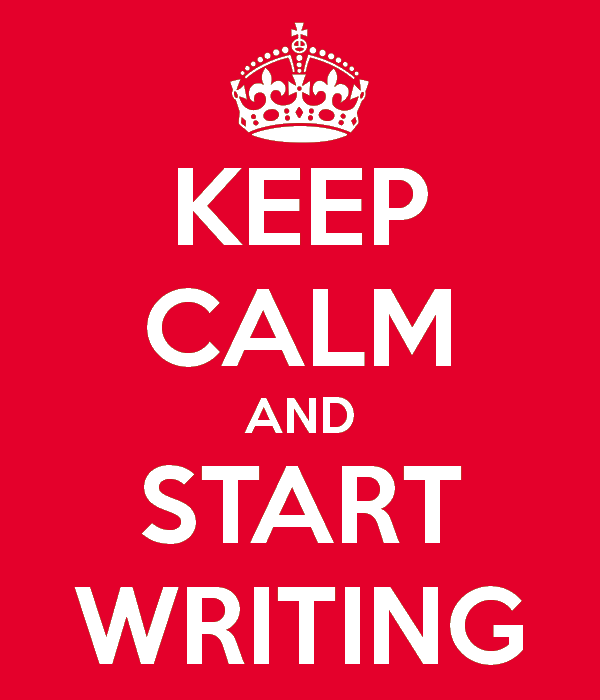
\includegraphics[scale=0.3]{obrazky-figures/keep-calm.png}
		\caption{Vygenerovaný půdorys oblasti}
	\end{subfigure}
	\begin{subfigure}{0.475\textwidth}
		\centering
		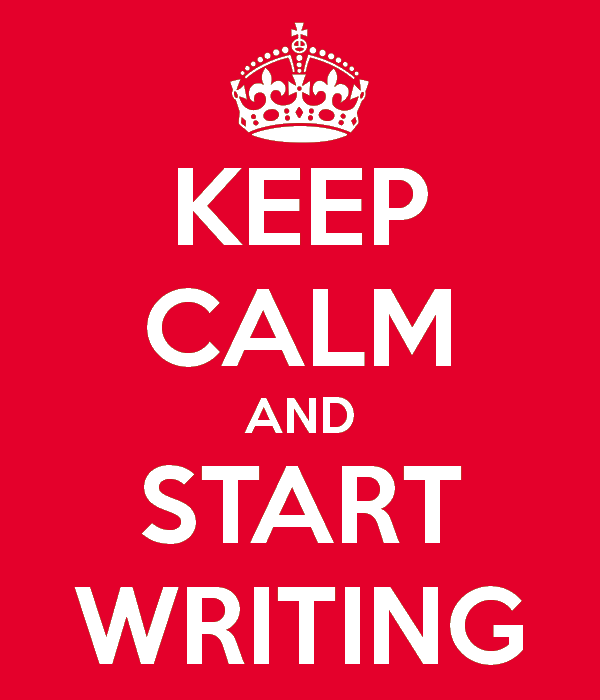
\includegraphics[scale=0.3]{obrazky-figures/keep-calm.png}
		\caption{Přidané stromy k půdorysu}
	\end{subfigure}
	\caption{Na obrázcích jsou vidět různé postupy generování obsahu, na obrázku a je vygenerovaný půdorys oblasti i s mořem a skálou, na obrázku b se k tomu přidaly stromy}
\end{figure}

	



\todo{informace o všemožných známých metodách procedurálního generování}

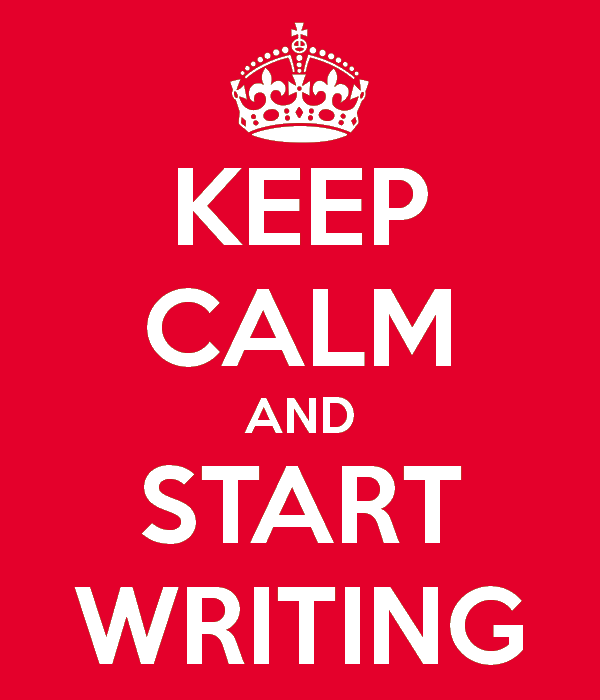
\includegraphics[scale=0.3]{obrazky-figures/keep-calm.png}

\textcolor{gray}{\blindtext[4]}


\subsubsection{Porovnání metod}
\todo{porovnání jednotlivých metod}
\textcolor{gray}{\blindtext[8]}

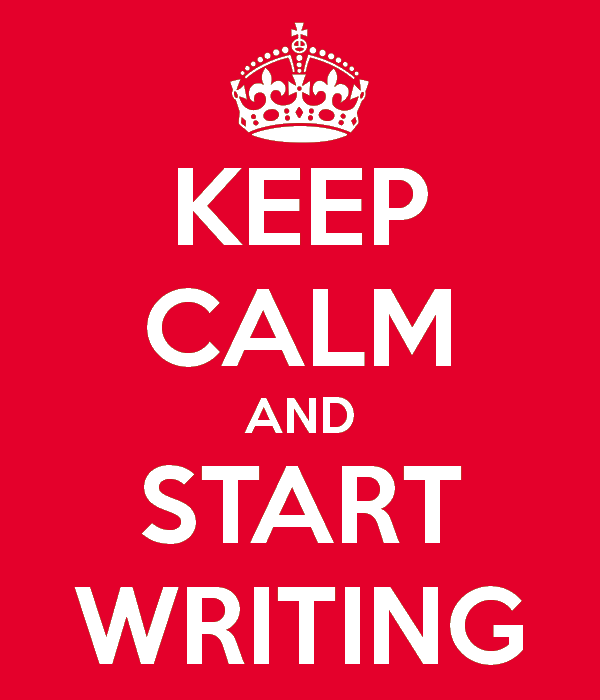
\includegraphics[scale=0.3]{obrazky-figures/keep-calm.png}

\textcolor{gray}{\blindtext[23]}


\section{2D hry}

\todo{popis hry}
\textcolor{gray}{\blindtext[18]}
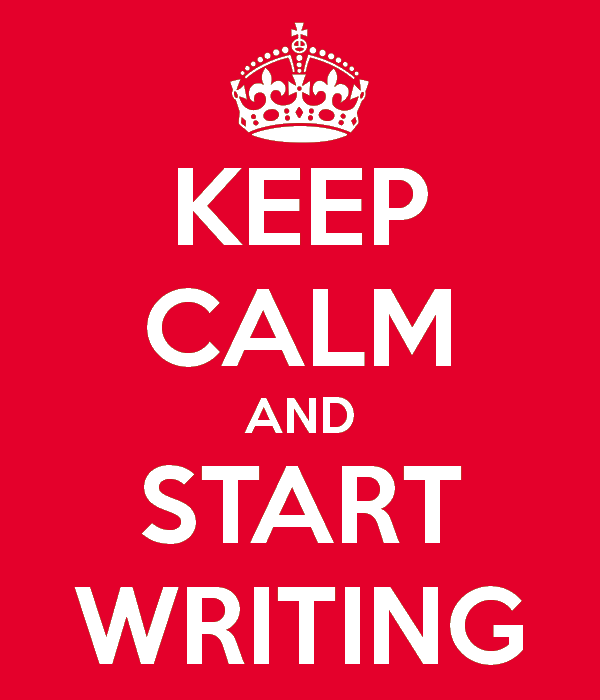
\includegraphics[scale=0.3]{obrazky-figures/keep-calm.png}

\subsection{Enginy na vývoj her}
\label{enginy}
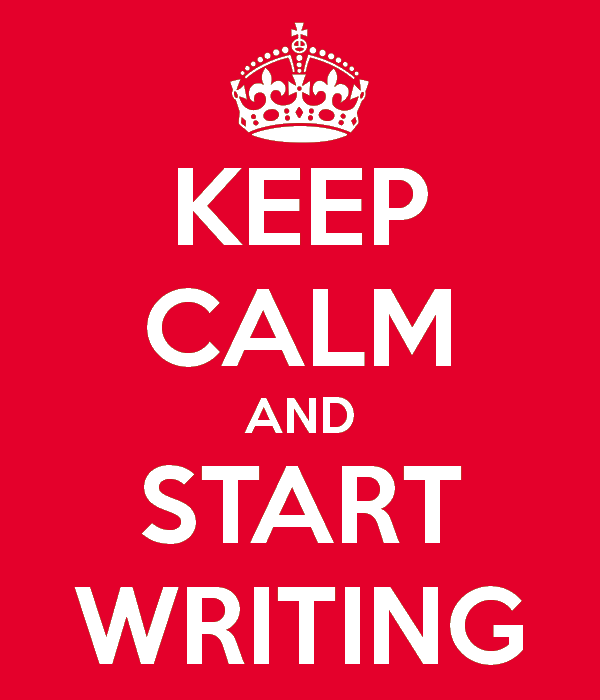
\includegraphics[scale=0.3]{obrazky-figures/keep-calm.png}

\textcolor{gray}{\blindtext[18]}

\chapter{Návrh řešení}
\label{solution}
\textcolor{gray}{\blindtext[2]}
\textcolor{gray}{\blindtext[46]}

\section{Vybraná metoda generování}
\todo{podrobnější popis metody, výhody, nevýhody}
\textcolor{gray}{\blindtext[46]}

\chapter{Realizace, experimenty a vyhodnocení}
\label{realization}
\textcolor{gray}{\blindtext[94]}

\chapter{Závěr}
\label{end}
\textcolor{gray}{\blindtext[4]}